\section{Student Relationships in Discussion Forums}

\begin{wrapfigure}{r}{0.6\linewidth}
  \begin{center}
    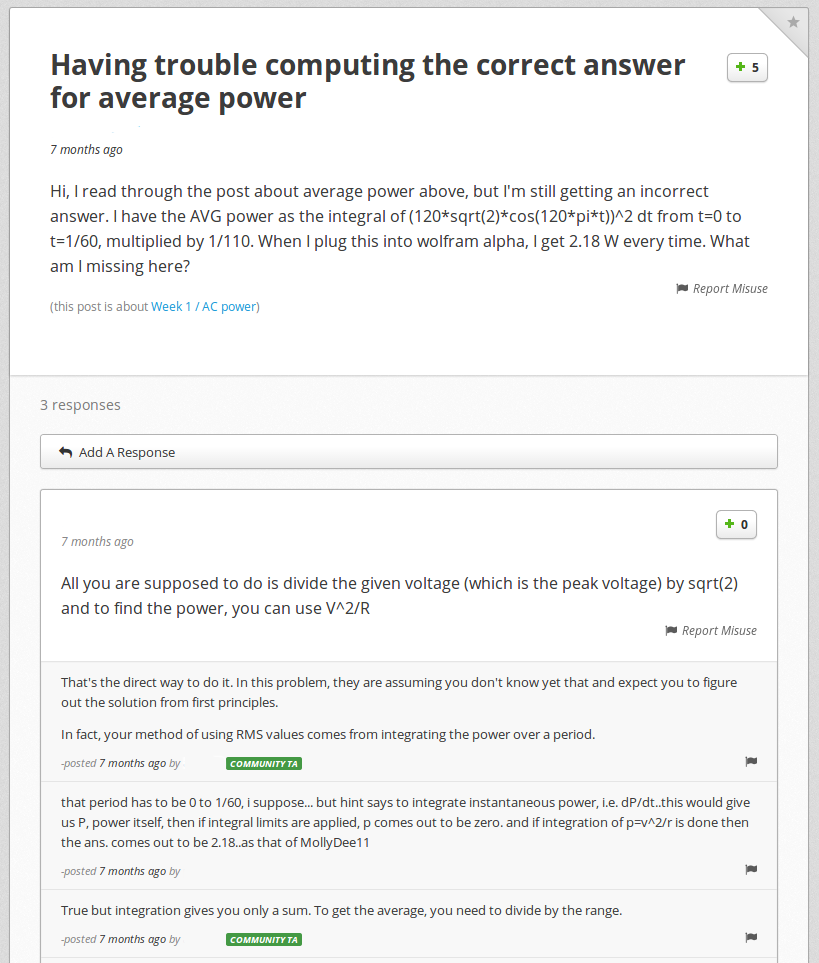
\includegraphics[width=1\linewidth]{forum_example.png}
    \caption{An example thread from 6.002x Spring 2014, which is currently being offered.}
    \label{forum}
  \end{center}
\end{wrapfigure}

Students interact in the discussion forums. Because of this, we can infer inter-student relationships based on a corpus of forum posts. 

The discussion forms we consider in this paper are organized as a collections of threads. Within a thread, students have the opportunity to converse with each other on a common topic. Figure \ref{forum} is an example thread from a class currently being offered on edX.

We rely on the thread structure of the conversations to determine student relationships. A thread is a hierarchy of posts where every post besides the first has a parent post that it is associated with. The parent/child relationship is interpreted as the child post being a reply to the parent. We use this interpretation to say author of a child post has interacted with the author the parent post. We only consider the immediate parent. 

We consider two students to be related if they interact in a thread. The strength of this relationship is determined by how often one student replies to another. The idea is that the more often we find one student replying to another, the more likely are in the same communitiy.

Using this understanding of how students who post on the forum are related, we present the idea of an Interaction Graph. 

\subsection{Interaction Graph}
\begin{figure}[h]
  \centering
  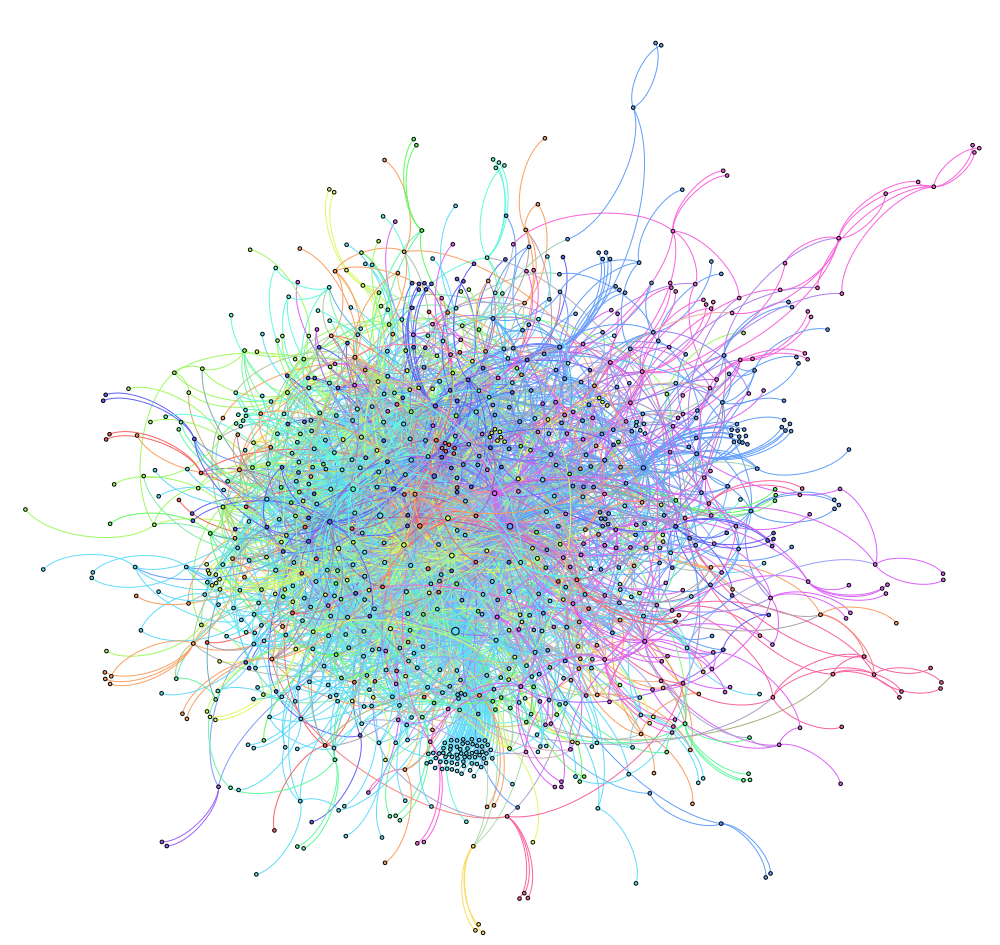
\includegraphics[width=.7\linewidth]{interaction_graph.png}
  \caption{This is a visualization of the Interaction Graph for 6.002x Fall 2012. This graph has 2163 students who made 6902 posts.}
  \label{interactions}
\end{figure}

In an Interaction Graph, each vertex represents a student in the class. For two students $i$ and $j$, the graph has a directed edge from $i$ to $j$ if $i$ has made a comment in direct reply to $j$. The edge between $i$ and $j$ is weighted by the number of times that $i$ directly replied to $j$ across all threads in the forum. We use this directed and weighted model to preserve as much information as possible about the the original forum interactions. Only students who are involved in a thread with at least one reply are considered. Figure \ref{interactions} shows what the graph of student interactions looks like for 6.002x offered in Fall 2012.